\documentclass[a4paper,11pt]{article}
\usepackage[utf8]{inputenc}
\usepackage[T1]{fontenc}
\usepackage[english]{babel}
\usepackage{newtxtext,newtxmath}
\usepackage[a4paper,margin=1in,headheight=14pt]{geometry}
\usepackage{graphicx}
\usepackage{booktabs,longtable,tabularx,array}
\usepackage{enumitem}
\usepackage{titlesec}
\usepackage{fancyhdr}
\usepackage{hyperref}
\usepackage{tikz}
\usetikzlibrary{arrows.meta,positioning,shapes.geometric}
\usepackage{caption}
\usepackage{microtype}
\usepackage{etoolbox}
\setcounter{tocdepth}{2}
\emergencystretch=3em
\hypersetup{colorlinks=true,linkcolor=black,citecolor=black,urlcolor=blue}
\setlength{\parindent}{1.25cm}
\setlength{\parskip}{3pt}
\setlist{nosep,leftmargin=*}
\setlength{\headheight}{16pt}
\titleformat{\section}{\normalfont\Large\bfseries}{\thesection}{0.7em}{}
\titleformat{\subsection}{\normalfont\large\bfseries}{\thesubsection}{0.7em}{}
\pagestyle{fancy}\fancyhf{}\lhead{Master’s Research Proposal}\rhead{Adaptive Evidence Acquisition}\cfoot{\thepage}

% One-file edition: the optional university image will appear if download.jpg exists.
\begin{document}
\hypersetup{pageanchor=false}
\begin{titlepage}\centering
\IfFileExists{download.jpg}{\includegraphics[width=0.22\textwidth]{download.jpg}\par}{}\vspace{0.6cm}
{\large Sana’a University\par}
{\large Faculty of Computer and Information Technology\par}
{\large Department of Cyber Security\par}
{\LARGE\bfseries Adaptive Evidence Acquisition for AI-Assisted Threat Hunting\par}
{\LARGE\bfseries Under Limited Telemetry\par}
\vspace{0.4cm}{\large Master’s Research Proposal\par}
\vspace{0.3cm}Author: ENG. Anas Nadhim Aldubai\par
\vspace{0.3cm}Supervisor: Assoc. Prof. Dr. Ahmed Al-Shalabi\par
\vspace{0.3cm}October 13, 2026\par
\end{titlepage}
\hypersetup{pageanchor=true}
\section*{Abstract}
Threat hunting is a hypothesis driven activity in which analysts are searching for adversary activity that automated detection has not reported. In reality hunters don't work with complete data sets. Logs can be missing, logs can be delayed, logs can be inconsistently collected across the different systems and logs can simply be outside of the scope of what is being monitored. Every additional query or collection action has a cost in terms of analyst time, processing, delay and access. Much of the existing work on alert triage, provenance based correlation and attack reconstruction operates on the assumption that the relevant telemetry is already available and provides little support in the decision of which evidence to go out and get next when it isn't. This proposal looks at an adaptive, AI assisted evidence acquisition approach. Given an evolving investigation state (threat hypotheses, observations and open questions) the approach will select the next evidence source or query by taking into account expected information value, relevance to the investigation objective, uncertainty reduction, collection and processing cost, delay, availability and access restrictions. It explicitly makes the distinction between evidence of absence and absence of evidence so that missing telemetry is never treated as evidence of benign or malicious activity. The work will be conducted in a Design Science Research manner with an artefact to be designed and prototyped and then evaluated in a series of controlled experiments with simulated telemetry limitations against two baselines (fixed priority and random evidence selection). The planned evaluation measures are hypothesis assessment quality, investigation cost, evidence efficiency, uncertainty reduction, calibration, unsupported conclusion rate, robustness and decision traceability. The prototype is intended to be a tool to support rather than replace the analyst. There is also a plan to conduct an applicability assessment in the Yemen focused operational context. No experiments have been carried out to date and no performance claims are being made.
\par
Keywords: threat hunting; evidence acquisition; limited telemetry; value of information; uncertainty; explainable AI; design science research.
\newpage
\tableofcontents
\clearpage
% Preserved original, manually typed table of contents (not printed):
% \section*{Contents}
% 1 Introduction 1\par
% 1.1 Background and Motivation… 1 1.2 Problem Statement… 1 1.3 Research Aim and Scope… 1 1.4 Expected Contributions… 1 1.5 Structure of the Proposal… 2\par
% 2 Literature Review 2\par
% 2.1 Threat Hunting Workflows and Security Telemetry… 2 2.2 Event Correlation and Attack Reconstruction… 2 2.3 Value of Information and Active Information Acquisition… 2 2.4 Active Learning and Sequential Decision-Making… 3 2.5 Uncertainty Estimation and Missing Data… 3 2.6 Explainable AI and Decision Traceability… 3 2.7 Operational Constraints… 3 2.8 Comparative Summary and Research Gap… 3\par
% 3 Research Questions, Objectives, and Hypotheses 4\par
% 3.1 Research Questions… 4 3.2 Objectives… 4 3.3 Hypotheses… 5 3.4 Alignment of Questions, Objectives, and Evaluation… 5\par
% 4 Evidence-Acquisition Framework 5\par
% 4.1 Investigation State... 5 4.2 Candidate Evidence Requests... 6 4.3 Interpretation of Missing Telemetry... 6 4.4 Selection Criteria... 6 4.5 State Update and Traceability... 7\par
% 5 Methodology 7\par
% 5.1 Research Design… 7 5.2 Phases… 7 5.3 Prototype Requirements… 7 5.4 Applicability Assessment… 8\par
% 6 Experimental Evaluation 8\par
% 6.1 Compared Methods… 8 6.2 Metrics… 8 6.3 Experimental Procedure and Analysis… 8 6.4 Threats to Validity… 9\par
% 7 Data, Telemetry Degradation, and Reproducibility 9\par
% 7.1 Dataset Selection Criteria... 9 7.2 Telemetry Degradation Simulation... 9 7.3 Scope of Simulated Limitations... 9 7.4 Reproducibility Procedures... 9\par
% 8 Ethics and Responsible AI 10\par
% 9 Work Plan, Risks, and Limitations 10\par
% 9.1 Work Plan… 10 9.2 Risks and Mitigation… 10 9.3 Limitations… 11\par
% 10 Conclusion 11\par
% A Working Terminology 13\par
% B Scenario Specification Template 14\par
% \newpage

\section{Introduction}
\subsection{Background and Motivation}
Threat hunting complements automated detection by actively looking for adversary behaviour that rules and signatures haven't picked up on (Lee and Bianco, 2016). A hunt generally begins with a hypothesis, e.g. that a particular technique from a knowledge base such as MITRE ATT\&CK (Strom et al., 2018) has been used in the environment, and then proceeds by querying the telemetry to either confirm, refine or dismiss that hypothesis. The quality of the outcome is very much dependent on what questions you're asking, in what order and against what data sources. In the real world you are of course constrained by operational reality. Log management guidance has been around for a long time and has always acknowledged that collection, retention and coverage are very uneven across systems (Kent and Souppaya, 2006). There's also a wealth of research on Security Operations Centre (SOC) operations which speaks to the reality of resource pressure, tool sprawl and analyst burnout (Kokulu et al., 2019; Alahmadi et al., 2022). In practice a hunter is often in a situation where the most useful data source is either not available, is too late, is too expensive to query or is simply not accessible. The cheaper sources will provide only a partial answer. The choice of what to query next is therefore a sequential decision under uncertainty and cost, and in practice is usually just guided by analyst experience and fixed playbooks rather than by an explicit, auditable policy.\par
\subsection{Problem Statement}
The current state of AI-assisted security analysis is very much focused on classification and correlation of the data that's already there. The question of what additional evidence an investigation should go out and collect when telemetry is sparse has received far less attention and the way in which conclusions should be qualified in the absence of that evidence has not been well considered. Without such assistance the analyst may well end up spending time on low value queries, miss out on cheaper sources of information that would have actually resolved the key uncertainty or reach conclusions that are simply not supported by the evidence at hand. A very serious error to make is to treat the absence of a log as a finding; the absence of a log may simply be a reflection of a coverage gap rather than the absence of an event.\par
\subsection{Research Aim and Scope}
The aim is to design and evaluate an adaptive evidence acquisition approach to help analysts decide on the next evidence source or query to investigate given limited telemetry, with uncertainty and the provenance of every conclusion being explicit. The scope is intentionally narrow. We are looking at evidence selection and investigation state reasoning within a single investigation only. This is not a detection model, not a full SIEM replacement, not automated response and not autonomous decision making. Evaluation will be performed using datasets and simulated telemetry constraints. Live production environments are not in scope.\par
\subsection{Expected Contributions}
The research intends to contribute the following, subject to the literature comparison and the experimental outcomes:\par
An adaptive evidence acquisition model which represents the hypotheses, observations, open questions and telemetry source status in an updateable investigation state.\par
A cost aware evidence selection policy which ranks the candidate evidence requests on expected value against collection cost, delay, availability and access constraints.\par
Uncertainty aware threat hunting assistance, including an explicit treatment of missing telemetry and calibrated/traceable conclusions.\par
A reproducible evaluation framework with parameterised telemetry degradation, defined baselines and metrics.\par
A Yemen specific applicability assessment of the approach's operational assumptions. No novelty is asserted at this stage as it will only be apparent following the systematic comparison with the related work described in Section 2. Similarly no claim of superiority over existing approaches is made without experimental evidence.\par
\subsection{Structure of the Proposal}
Section 2 is the related work; Section 3 contains the research questions, objectives and hypotheses; Section 4 defines the evidence acquisition framework; Sections 5-7 detail the methodology, evaluation design and data and reproducibility plan; Section 8 is on ethics; Section 9 is the work plan, risks and limitations.\par
\section{Literature Review}
This review is structured by the research areas upon which the proposal is based. It is a preliminary critical review based on the foundational and highly cited literature. A systematic search and screening will be carried out in the first phase of the project (Section 9) prior to any claim of novelty being made.\par
\subsection{Threat Hunting Workflows and Security Telemetry}
Hypothesis driven hunting is typically described as a cycle of hypothesising, investigating via the data at hand, finding the patterns and then feeding that back into the detection (Lee and Bianco, 2016). ATT\&CK provides a common language of adversary TTPs that hunters use to formulate their hypotheses (Strom et al., 2018). The descriptions are largely procedural in nature in that they tell you what to hunt for, they don't really give you any formal guidance on how to prioritise your data requests when you have a range of sources that vary in cost and availability. Telemetry itself is a very heterogeneous thing. Log management guidance is well aware of the variety of sources, formats and retention periods (Kent and Souppaya, 2006) and practitioner studies have identified the problems of gaps, noise and coverage in the operational centres (Kokulu et al., 2019; Alahmadi et al., 2022). These are the problems that the hypothesis driven hunting approach is trying to address, but the existing descriptions don't actually model the telemetry limitations as an explicit input to the investigation strategy.\par
\subsection{Event Correlation and Attack Reconstruction}
There's a fair bit of work that takes low level events and turns them into attack narratives. SLEUTH takes audit data and reconstructs attack scenarios (Hossain et al., 2017); HOLMES looks at suspicious information flows and correlates them to identify advanced persistent threats (Milajerdi et al., 2019); NoDoze uses provenance to help prioritise alerts and thereby reduce alert fatigue (Hassan et al., 2019); Hopper models and detects lateral movement from authentication logs (Ho et al., 2021). All of these systems illustrate the benefit of some form of structured correlation, albeit they all work on the telemetry that has already been gathered. They don't make a decision as to what further evidence to request and they don't in any systematic way differentiate between a negative that is confirmed and a negative that is simply not observed.\par
\subsection{Value of Information and Active Information Acquisition}
Value of information theory formalises the value of getting information prior to making a decision (Howard, 1966). In the context of graphical models there has been a good deal of work on the selection of observations to maximise expected utility (Krause and Guestrin, 2009) and adaptive submodularity provides performance guarantees for sequential selection under certain conditions (Golovin and Krause, 2011). Partially observable decision processes provide a general framework for acting when the state is not directly observable (Kaelbling et al., 1998; Sutton and Barto, 2018). These results provide a principled basis for evidence selection, albeit in a rather abstract form.\par
Assumptions (submodularity, known observation models, tractable state spaces etc) need not hold in a security investigation and applications to threat hunting under explicit availability and access constraints as far as the author is aware are very limited. That would require the systematic search outlined above.\par
\subsection{Active Learning and Sequential Decision-Making}
Active learning is the process of selecting which unlabelled instances to query in order to improve the model efficiently (Settles, 2009). The hunting analogy is only partial in this context: active learning is typically concerned with maximising the accuracy of the model over a large number of labels whereas a hunt is concerned with maximising the assessment of a small number of hypotheses in a single case. There are heterogeneous query costs and the possibility that a query may simply not be answerable at all. The sequential decision literature (Sutton and Barto, 2018) provides policy formulations but it is utterly impractical to learn such policies by interacting with the real world in a live investigation. This in turn supports the idea of starting with explicit, inspectable selection criteria and then evaluating those in simulation.\par
\subsection{Uncertainty Estimation and Missing Data}
Decision support requires uncertainty that is meaningful. Epistemic and aleatoric uncertainty are different and require different responses (Hüllermeier and Waegeman, 2021; Kendall and Gal, 2017) with more evidence able to reduce the former but not the latter. Modern models are often badly calibrated (Guo et al., 2017) so you can't trust the confidence that they report without checking. The missing data literature makes a distinction between the different mechanisms by which data can go missing (Little and Rubin, 2019) and of course the axiom that "absence of evidence is not evidence of absence" (Altman and Bland, 1995) is very much relevant to logs. In threat hunting a missing record could mean the event didn't happen, the source didn't see it or the record is simply delayed. This proposal treats those as distinct states of the investigation rather than simply lumping them together.\par
\subsection{Explainable AI and Decision Traceability}
Explanation methods like SHAP (Lundberg and Lee, 2017) work by attributing the model output to the input features and the field has in fact called for well-defined notions and evaluation of what we mean by interpretability (Doshi-Velez and Kim, 2017). For the purposes of investigation though, feature attribution on its own is not enough. The analyst needs to know which evidence supports which conclusion, what was actually being asked for and why and what still remains to be resolved. The proposal is therefore focused on traceability of the investigation (the chain from request through to observation to belief update) rather than post-hoc model explanation.\par
\subsection{Operational Constraints}
Operational studies have demonstrated that analysts are up against the volume of alerts, tooling limitations and organisational constraints (Kokulu et al., 2019; Alahmadi et al., 2022). That means an approach which requires all the data, a huge compute budget or the ability to act autonomously would be very hard to implement. The studies point to cost and time as being the two key factors and to human in the loop as a necessary design element. There's likely to be very little literature specifically on resource constrained environments such as Yemen so the applicability assessment will be a mix of the existing literature, the assumptions we have and where appropriate expert input.\par
\subsection{Comparative Summary and Research Gap}
The body of work reviewed provides a good set of ingredients (correlation, value of information theory, calibration, explanation) but as far as this initial review goes the combination that is required here is not really addressed at all: the issue of selecting evidence sequentially in the course of threat hunting investigations whilst taking account of the above.\par
\par\noindent\textbf{Table 1: A preliminary comparison of the related approaches and the gap this proposal addresses.}\par
{\footnotesize\setlength{\tabcolsep}{3pt}\renewcommand{\arraystretch}{1.16}
\begin{longtable}{@{}p{0.16\linewidth}p{0.27\linewidth}p{0.23\linewidth}p{0.27\linewidth}@{}}
\toprule
Area & Representative works & Limitation for this problem & Proposed response \\
\midrule\endhead
Hunting workflows & Lee and Bianco (2016); Strom et al. (2018) & Procedural guidance; no request prioritisation & Rank candidate requests explicitly \\
\addlinespace[3pt]
Correlation and reconstruction & Hossain et al. (2017); Milajerdi et al. (2019); Hassan et al. (2019); Ho et al. (2021) & Assumes telemetry is already collected & Choose the next evidence to acquire \\
\addlinespace[3pt]
Value of information & Howard (1966); Krause and Guestrin (2009); Golovin and Krause (2011) & Assumptions may not fit hunting constraints & Include cost, delay, and access \\
\addlinespace[3pt]
Active learning and sequential decisions & Settles (2009); Kaelbling et al. (1998); Sutton and Barto (2018) & Model-centric; unavailable queries rarely modelled & Case-level selection with availability states \\
\addlinespace[3pt]
Uncertainty and missing data & Hüllermeier and Waegeman (2021); Guo et al. (2017); Little and Rubin (2019) & Not tied to log coverage semantics. & Distinguish verified negatives from missing evidence. \\
\addlinespace[3pt]
Explainability: & Lundberg and Lee (2017); Doshi-Velez and Kim (2017) & Feature-level explanations; weak investigation trace & Trace request–observation– update chain \\
\bottomrule
\end{longtable}
}
cost, delay, availability and access and reasoning explicitly about the missing telemetry. This is a working research gap (to be confirmed or otherwise by the systematic review).\par
\section{Research Questions, Objectives, and Hypotheses}
\subsection{Research Questions}
RQ1: How can an investigation state (threat hypotheses, observations, unresolved questions and telemetry source status) be represented such that the value of candidate evidence requests can be assessed in the face of limited telemetry?\par
RQ2: How can an evidence selection policy combine expected information value with collection cost, processing cost, delay, availability and access restrictions?\par
RQ3: Does the adaptive policy lead to improved hypothesis assessment quality and evidence efficiency relative to fixed priority and random selection under the constraints of controlled telemetry?\par
RQ4 How well calibrated, traceable and free from unsupported conclusions are the outputs of the approach when telemetry is missing, delayed or inconsistent?\par
RQ5: Under what operational conditions can the approach be applied in Yemen-centric environments and what assumptions restrict its applicability?\par
\subsection{Objectives}
O1 Define a formal representation of the investigation state and of telemetry source status (including the distinction between evidence of absence and absence of evidence) (RQ1).\par
O2: Design a cost-aware, uncertainty-aware evidence selection policy and justify its structure (RQ2).\par
O3: Implement a prototype and a parameterised telemetry degradation simulator (RQ2, RQ3).\par
O4 Evaluate the prototype against the two baselines using the defined metrics, with ablations (RQ3, RQ4).\par
O5: Analyse the applicability and assumptions in the Yemen-specific contexts (RQ5).\par
\subsection{Hypotheses}
The following are testable hypotheses (i.e. testable expectations), not findings. They will be accepted or rejected on the basis of the evaluation.\par
H1 At an equal investigation cost budget the adaptive policy achieves superior hypothesis assessment quality to both fixed priority and random selection.\par
H2 The adaptive policy achieves the required level of uncertainty reduction with fewer evidence requests than the baselines.\par
H3: Representing missing telemetry as distinct availability states results in a lower rate of unsupported conclusions than treating the missing data as negative evidence.\par
H4 The relative advantage of the adaptive policy is maintained (and will be quantified) as telemetry degradation increases. Each hypothesis is potentially refutable and negative or mixed results will be reported as such.\par
\subsection{Alignment of Questions, Objectives, and Evaluation}
\par\noindent\textbf{Table 2: Alignment of research questions, objectives, methodology and metrics.}\par
{\footnotesize\setlength{\tabcolsep}{3pt}\renewcommand{\arraystretch}{1.16}
\begin{longtable}{@{}p{0.07\linewidth}p{0.12\linewidth}p{0.37\linewidth}p{0.36\linewidth}@{}}
\toprule
RQ & Objective & Methodology component & Evaluation evidence \\
\midrule\endhead
RQ1 & O1 & Design phase: investigation-state model & Model specification; scenario-case coverage; traceability \\
\addlinespace[3pt]
RQ2 & O2, O3 & Design and prototype of selection policy & Ablation of policy factors; investigation cost \\
\addlinespace[3pt]
RQ3 & O3, O4 & Controlled experiments against two baselines & Hypothesis assessment quality; cost; evidence efficiency; uncertainty reduction (H1, H2, H4) \\
\addlinespace[3pt]
RQ4 & O4 & Calibration and traceability analysis & Calibration; unsupported conclusion rate; robustness; traceability (H3) \\
\addlinespace[3pt]
RQ5 & O5 & Applicability assessment & Documented assumptions and conditions; expert feedback where possible \\
\bottomrule
\end{longtable}
}
\section{Evidence-Acquisition Framework}
This section is the conceptual framework. The concrete representations and estimators are project design decisions and will be finalised and justified as part of the design process.\par
\subsection{Investigation State}
The investigation state at step t comprises four elements:\par
Threat hypotheses: candidate explanations of the activity under investigation (for example, the use of a particular ATT\&CK technique), each with an associated degree of belief and links to the supporting and contradicting observations.\par
Observations: evidence obtained to date, each with provenance (source, time, query) and a quality indicator.\par
Unresolved questions: questions which are specific and whose answers would allow you to discriminate between the hypotheses.\par
Telemetry source registry: for each source its coverage, collection and processing cost, expected delay, availability and access restrictions.\par
\subsection{Candidate Evidence Requests}
A candidate request is a query or collection action against a registered source which is intended to answer one or more of the open questions. Candidates are derived from the open questions and the source registry; the AI may suggest or rank candidates but each candidate must be linked to the question it is intended to answer so that the reasoning behind it is transparent.\par
\subsection{Interpretation of Missing Telemetry}
Every answer to a request is recorded in one of three states:\par
Present: a relevant record was located.\par
Evidence of absence: the source was operating and covering the relevant asset and period and there is no record. That is the only state which can count against a hypothesis and only to the extent that the source's coverage and reliability supports it.\par
Absence of evidence: the data were not available, were incomplete, were delayed or were outside the scope of monitoring. This leaves the associated question unanswered. It is not in itself evidence for or against any hypothesis and in particular is never read as evidence of malicious activity, attacker concealment or compromise. Whether an absence of data can be classified as evidence of absence is dependent on the coverage information. If the coverage information itself is uncertain then that uncertainty is carried forward in the framework rather than being assumed away.\par
\subsection{Selection Criteria}
The policy ranks candidate requests using the following criteria:\par
expected information value for the open questions (uncertainty reduction);\par
relevance to the investigation objective;\par
collection cost and processing cost;\par
expected delay;\par
source availability, including the probability that the request returns no usable answer;\par
Access restrictions and required authorisation. The way these criteria are combined (for instance as a weighted utility, a constrained selection or a lexicographic rule) is not specified in this proposal. No particular formula is assumed in advance: the method of combination will be selected as part of the design process, will be justified in the light of the literature on the value of information and will be subject to ablation so that the contribution of each criterion can be measured.\par
\subsection{State Update and Traceability}
After each acquisition the state is updated: beliefs are updated, questions are either resolved or re-formulated and the source registry is corrected where appropriate (i.e. where the answer provides a coverage/availability fact). Each update is logged in conjunction with the request that caused it so that the final state of belief can be traced back to the full evidence chain. The belief update mechanism is designed to be explicit and auditable (e.g. a probabilistic model over hypotheses); any learned or language model components that are used will be restricted to operations whose outputs can be checked against that chain. Figure 1 shows the loop. The\par
\begin{figure}[htbp]\centering
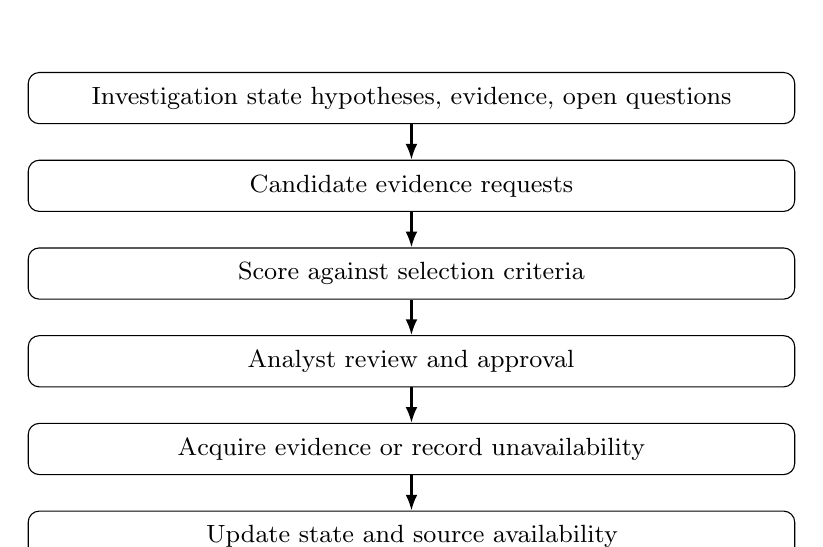
\begin{tikzpicture}[node distance=0.45cm, every node/.style={draw,rounded corners,align=center,text width=9.5cm,minimum height=0.65cm,font=\small}, arrow/.style={-{Latex[length=2mm]},thick}]
\node (n0) {Investigation state hypotheses, evidence, open questions};
\node (n1) [below=of n0] {Candidate evidence requests};
\draw[arrow] (n0) -- (n1);
\node (n2) [below=of n1] {Score against selection criteria};
\draw[arrow] (n1) -- (n2);
\node (n3) [below=of n2] {Analyst review and approval};
\draw[arrow] (n2) -- (n3);
\node (n4) [below=of n3] {Acquire evidence or record unavailability};
\draw[arrow] (n3) -- (n4);
\node (n5) [below=of n4] {Update state and source availability};
\draw[arrow] (n4) -- (n5);
\end{tikzpicture}
\caption{Conceptual adaptive evidence acquisition loop. The analyst remains in the loop prior to any request being executed.}
\end{figure}
The framework is a decision support element in that it will make recommendations as to requests and qualified conclusions and an analyst would then go on to review those.\par
\section{Methodology}
\subsection{Research Design}
The project incorporates three elements: Design Science Research, prototype development and controlled experimental evaluation. Design Science Research is the right methodology as the contribution is an artefact (a model and a policy) which is intended to solve a particular problem (Hevner et al., 2004). The process is in keeping with that described by Peffers et al. (2007) in that it involves problem identification, definition of objectives, design and development, demonstration, evaluation and communication.\par
\subsection{Phases}
Problem and literature phase: systematic literature search and screening according to the defined inclusion criteria, confirmation or refinement of the research gap (Section 2) and refinement of the requirements.\par
Design phase: specification of the investigation state, availability states and selection policy (O1, O2) including documented design alternatives and justification.\par
Prototype phase: implementation of the prototype and the telemetry degradation simulator (O3), versioned code and fixed random seeds.\par
Evaluation phase: controlled experiments, ablations and analysis (O4).\par
Applicability phase: assessment of Yemen-specific conditions and assumptions (O5).\par
\subsection{Prototype Requirements}
The prototype will (i) maintain the investigation state, (ii) generate and rank candidate requests, (iii) record each answer in one of the three states as described in Section 4.3, (iv) log all state changes for traceability and (v) present recommendations to a human. It will not perform any high impact actions on its own.\par
\subsection{Applicability Assessment}
The Yemen assessment will look at which of the approach's assumptions (e.g. availability of logging, query access, analyst capacity and tooling) are valid in the target contexts and which would need to be modified. Where there is very little published evidence, assumptions will be stated as such rather than as facts about the environment. Any engagement with practitioners will be carried out in accordance with the ethical safeguards of Section 8 and subject to institutional approval.\par
\section{Experimental Evaluation}
\subsection{Compared Methods}
Baseline 1: fixed priority selection. Candidate requests are taken in a pre-defined priority order (e.g. a playbook style ordering) with no adaptation to the evolving state. Baseline 2: random selection. Candidate requests are chosen uniformly at random from the set of those currently permitted, over many seeds. Proposed method: the adaptive cost-aware policy of Section 4. All methods use the same candidate set, the same belief update mechanism and the same investigation budget so any differences are due to the selection policy. Ablated versions of the proposed method (removing in turn the cost, delay, availability and uncertainty components and the three state treatment of absence) will quantify the contribution of each component.\par
\subsection{Metrics}
% SOURCE ALERT: In the supplied text, the metrics table is merged with sections 6.3, 6.4, 7 and 8.
% Original spellings, duplicated fragments, and unfinished words are retained on purpose.

Table 3: Planned evaluation metrics. Operational definitions will be finalised in Investigation cost. Cumulative collection cost, processing cost and delay consumed. RQ3, H1. Evidence efficiency. Assessment quality or uncertainty reduction achieved per unit cost or per request.cost Cumulative collection cost, processing cost, and delay consumed RQ3, H1 Evidence efficiency Assessment quality or uncertainty reduction obtained per unit cost or per request\par
RQ3, H2\par
Uncertainty reduction Change in uncertainty over hypotheses between start and end of investigation\par
RQ3, H2\par
Calibration Correspondence between stated confidence and observed correctness, using standard calibration measures (Guo et al., 2017)\par
RQ4\par
Unsupported-conclusion rate\par
Share of conclusions not backed by sufficient recorded evidence, including conclusions that rely on absence of evidence alone\par
RQ4, H3\par
Robustness Stability of measures as missing, delayed, or inconsistent telemetry incr\subsection{Experimental Procedure and Analysis}
Each scenario is run under each method and each degradation condition with multiple seeds. The comparisons are paired by scenario and condition. Results will be reported with effect sizes and confidence intervals and significance will be assessed via appropriate non-parametric paired tests or bootstrap procedures (with correction for multiple comparisons). All planned analyses (including any that may be detrimental to the proposed method) will be pre-specified prior to the final experiments being run. The expected improvements are hypotheses and will not be reported as results. including those that may d\subsection{Threats to Validity}
Internal validity: the shared implementation components could be a source of confounding with respect to the policy effects (this is mitigated by the common infrastructure and the ablation studies). Construct validity: the metrics are proxies for analyst benefit; the traceability and cost metrics are derived from design choices which will be documented. External validity: the scenarios and simulated degradations are quite limited and do not cover the full range of real environments. Ground truth validity: the scenario labels may be incomplete and may be biased in some way by how the scenarios were constructed.nd simulated degradation are limited and do not cover all real environments. Ground-tr\section{Data, Telemetry Degradation, and Reproducibility}
\subsection{Dataset Selection Criteria}
Candidate datasets and scenarios must: (i) have multiple telemetry sources with timestamps so that different evidence requests are meaningful; (ii) have sufficient ground truth to allow hypotheses to be labelled; (iii) be publicly available or otherwise legally and ethically usable for research; (iv) allow evidence requests to be simulated as queries against the data; and (v) be well documented so that they can be reproduced. The Los Alamos National Laboratory multi-source enterprise event data (Kent, 2015) is one such candidate. CIC-IDS2017 (Sharafaldin et al., 2018) is a possible candidate for a secondary, single source test though it has the major limitation of having very little multi-source structure. If the public data don't have the required structure then ATT\&CK-aligned scenarios will be built on top of them with documented ground truth (Appendix B). The final dataset selection with justification and known limitations will be captured as part of the design phase. be constructed on top of them with docuDegradation is applied to the data that's available to the investigation, not to the ground truth. The simulator is parameterised across four dimensions:elemetry Degradation Simulation\par
\subsection{Telemetry Degradation Simulation}
Degradation is applied to the data available to the investigation, not to the ground truth. The simulator is parameterised along four dimensions:\par
missing events: removal of events at defined rates and patterns, including whole-sourcAccess restrictions: sources that can't be queried at all, or only at increased cost. The simulator will record which absences are true negatives (the source was operating and nothing happened) and which are coverage gaps so that the distinction of Section 4.3 can be scored. The degradation levels and patterns will be justified by the missing data literature (Little and Rubin, 2019) and by the operational reports that are available and will be fixed in a config file.evels and patterns will be justified b\subsection{Scope of Simulated Limitations}
The simulated constraints are under experimental conditions. They do not represent all real world security environments and results obtained under them will not be generalisable beyond those conditions.d limitations are experimental con\subsection{Reproducibility Procedures}
The project will: publish the source code and configuration under version control; fix and report the random seeds; record the software versions and environment specifications; document the dataset versions and the preprocessing steps; release the scenario definitions and degradation configurations. Where a dataset's licence prevents redistribution the scripts will download it from the original source. Reproducibility is of course limited by the availability of third party datasets and any non-deterministic elements; these limitations will be reported.l fetch it from its original so\section{Ethics and Responsible AI}
Authorised data access: only publicly available data, synthetic data or data for which explicit authorisation (and where applicable institutional ethics approval) has been obtained will be used. No system will be accessed or tested without permission. wPrivacy protection: security telemetry may contain personal data (user identifiers, addresses, activity traces). Where possible the data will be minimised, anonymised or pseudonymised, stored securely and not re-distributed beyond the licence terms. The work will be guided by the principles of the Menlo Report on ICT research ethics (Dittrich and Kenneally, 2012).osResponsible security data handling: no exploit or attack tooling is part of the contribution. The scenario descriptions will be at a level appropriate for evaluation and will not contain operational attack instructions. oHuman oversight: the system is there to assist analysts and will not make any critical security decisions automatically. The recommendations are advisory, will be accompanied by their evidence chain and uncertainty and will require human review prior to any request being executed or any conclusion being acted upon. This is in line with the emphasis on accountability and transparency in the NIST guidance on risk management for AI (NIST, 2023).isTransparency regarding limitations: the reported results will state the conditions under which they hold and failures and negative results will be reported.ndards     and Technology, 2023).\par
Transparency about Table 4: Proposed work plan. Durations are relative and will be aligned to the programme calendar.esults will be reported.\par
\section{Work Plan, Risks, and Limitations}
\subsection{Work Plan}
Problem and literature: systematic review; confirmed gap; refined requirements. Early Design Investigation: state model; selection policy specification. Early to mid Prototype: prototype; degradation simulator; scenario set. Mid Evaluation: experiments; ablations; statistical analysis. Mid to late: applicability (Yemen focused assessment). Late: writing and submission (thesis, code and data release) throughout and then finally.valuation Experiments; ablat\subsection{Risks and Mitigation}
No suitable public multi-source dataset: we'd have to construct the ATT\&CK-aligned scenarios from the available data and we'd have to state that that's a limitation.ThGap already addressed in the literature: the systematic review may indicate that the contribution is in fact already covered by the existing work. The framing would then be changed to a comparison or an extension and the novelty claim would be dropped. sPolicy offers no advantage over the baselines (the finding is reported). We then go on to analyse the conditions under which fixed or random selection will be sufficient.nsPoorly calibrated belief updates: perform explicit, auditable updating and calibration analysis prior to ascribing the results to the policy.fiVery limited access to practitioners to assess the applicability: we're reliant on the literature and on the documented assumptions (all of which are clearly flagged).fore     attributin\subsection{Limitations}
The evaluation is based on datasets and simulated degradation and does not constitute an assessment of performance in actual operations. Ground truth for the hypotheses is likely to be incomplete. The approach is about evidence selection in an investigation rather than detection and is predicated on the accuracy of the source registry (coverage, cost, delay). The Yemen assessment will be constrained by the amount of published evidence available and by access to the practitioners. The literature review in this version is very preliminary and the novelty of the contribution is not established.y the availabilit\section{Conclusion}
This proposal is concerned with how an investigation can select its next piece of evidence when telemetry is sparse, expensive or simply not available at all and how to avoid the situation where missing telemetry is interpreted as a finding. It details the investigation state framework, the selection criteria, the baselines and metrics, the way in which telemetry sparsity will be simulated and the ethical considerations. The key claims are all hypotheses to be tested and the stated gap and contributions are all provisional until the systematic literature review and the experiments have been carried out.al claims are % SOURCE ALERT: The original references are fused together; all source words are retained.
\section*{References}
\addcontentsline{toc}{section}{References}
[1] Bushra A. Alahmadi, Louise Axon and Ivan Martinovic. 99\% false positives: A qualitative study of SOC analysts' perspectives on security alarms. In 31st USENIX Security Symposium, 2022.A. Alahmadi, Louise Axon, and Ivan Martinovic. 99\% false positives: A qualitative study of SOC analysts’ perspectives on security alarms. In 31st USENIX Security Symposium, 2022.
[2] Douglas G. Altman and J. Martin Bland. Absence of evidence is not evidence of absence. BMJ, 311(7003):485, 1995.\par
[3] David Dittrich and Erin Kenneally. The Menlo report: Ethical principles guiding information and communication technology r[5] Daniel Golovin and Andreas Krause. Adaptive submodularity: Theory and applications in active learning and stochastic optimisation. Journal of Artificial Intelligence Research, 42:427–486, 2011.an[6] Chuan Guo, Geoff Pleiss, Yu Sun and Kilian Q. Weinberger. On calibration of modern neural networks. In Proceedings of the 34th International Conference on Machine Learning, volume 70 of Proceedings of Machine Learning Research, pages 1321–1330, 2017. o[7] Wajih Ul Hassan, Shengjian Guo, Ding Li, Zhengzhang Chen, Kangkook Jee, Zhichun Li and Adam Bates. NoDoze: Combatting threat alert fatigue with automated provenance triage. In Network and Distributed System Security Symposium (NDSS), 2019.ko[8] Alan R. Hevner, Salvatore T. March, Jinsoo Park and Sudha Ram. Design science in information systems research. MIS Quarterly, 28(1):75-105, 2004.ty[9] Grant Ho, Mayank Dhiman, Devdatta Akhawe, Vern Paxson, Stefan Savage, Geoffrey M. Voelker and David Wagner. Hopper: Modeling and detecting lateral movement. In 30th USENIX Security Symposium, 2021.ma[10] Md Nahid Hossain, Sadegh M. Milajerdi, Junao Wang, Birhanu Eshete, Rigel Gjomemo, R. Sekar, Scott D. Stoller and V. N. Venkatakrishnan. SLEUTH: Real-time attack scenario reconstruction from COTS audit data. In 26th USENIX Security Symposium, 2017.el Gjomemo, R. Sekar, Scott D. Stoller, and V. N. Venkatakrishnan. SLEUTH: Real-time attack scenario reconstruction from COTS audit data. In 26th USENIX Security Symposium, 2017.\par
[11] Ronald A. Howard. Information value theory. IEEE Transactions on Systems Science and Cybernetics, 2(1):22–26, 1966.\par
[12][13] Leslie Pack Kaelbling, Michael L. Littman and Anthony R. Cassandra. Planning and acting in partially observable stochastic domains. Artificial Intelligence, 101(1–2):99–134, 1998.slie Pack Kaelbling, Michael L. Littman, and Anthony R. Cassandra. Planning and acting in partially observable stochastic domains. Artificial Intelligence, 101(1–2):99–134, 1998.\par
[14] Alex Kendall and Yarin Gal. What uncertainties do we need in Bayesian deep learning for computer vision? In Advan[16] Karen Kent and Murugiah Souppaya, Guide to Computer Security Log Management, Special Publication 800-92, National Institute of Standards and Technology, 2006.at[17] Faris Bugra Kokulu, Ananta Soneji, Tiffany Bao, Yan Shoshitaishvili, Ziming Zhao, Adam Doupé and Gail-Joon Ahn. Matched and mismatched SOCs: A qualitative study on security operations centre issues. In Proceedings of the ACM SIGSAC Conference on Computer and Communications Security (CCS), 2019.ed and mismatched SOCs: A qualitative study on security operations center issues. In Proceedings of the ACM SIGSAC Conference on Computer and Communications Security (CCS), 2019.\par
[18] Andreas Krause and Carlos Guestrin. Optimal value of information in graphical models. Journal of Artificial Intelligence Research, 35:557–591, 2009.\par
[19] Robert M. Lee and David Bianco. Generating hypotheses for successful threat hunting. White paper, SANS Institute, 2016.\par
[20] Roderick J. A. Little and Donald B. Rubin. Statistical Analysis with Missing Data. Wiley[22] Sadegh M. Milajerdi, Rigel Gjomemo, Birhanu Eshete, R. Sekar and V. N. Venkatakrishnan. HOLMES: Real-time APT detection through correlation of suspicious information flows. In IEEE Symposium on Security and Privacy, 2019.Eshete, R. Sekar, and V. N. Venkatakrishnan. HOLMES: Real-time APT detection through correlation of suspicious information flows. In IEEE Symposium[24] Ken Peffers, Tuure Tuunanen, Marcus A. Rothenberger and Samir Chatterjee. A design science research methodology for information systems research. Journal of Management Information Systems, 24(3):45-77, 2007.arcus A. Rothenberger, and Samir Chatterjee. A design science research methodology for information systems research. Journal of Managemen[26] Iman Sharafaldin, Arash Habibi Lashkari and Ali A. Ghorbani. Toward generating a new intrusion detection dataset and intrusion traffic characterization. In Proceedings of the 4th International Conference on Information Systems Security and Privacy (ICISSP), 2018.in[27] Blake E. Strom, Andy Applebaum, Doug P. Miller, Kathryn C. Nickels, Adam G. Pennington and Cody B. Thomas. MITRE ATT\&CK: Design and philosophy. Technical report, The MITRE Corporation, 2018.m, Andy Applebaum, Doug P. Miller, Kathryn C. Nickels, Adam G. Pennington, and Cody B. Thomas. MITRE ATT\&CK: Design and philosophy. Technical\section*{A Working Terminology}
\addcontentsline{toc}{section}{A Working Terminology}
Telemetry records produced by the monitored systems (authentication, process, network, DNS logs etc) which can be queried during an investigation.\par
Evidence of absence: a source with proper coverage has confirmed the event didn't happen.s,No evidence available - data simply weren't there (unavailable, incomplete, delayed or outside of coverage) so the issue remains open. cEvidence request: a query or collection action against a telemetry source.caInvestigation state: The current hypotheses, observations, outstanding questions and source registry..\par
Unsupported conclusion: a conclusion not supported by sufficient recorded evidence (including one based solely on absence of evidence).s, unresolved questions, and source registry.\par
Unsupported conclusion A conclusion not backed by sufficient recorded evidence, including one resting on absence of evidence alone.\par
\section*{B Scenario Specification Template}
\addcontentsline{toc}{section}{B Scenario Specification Template}
Each evaluation scenario will be documented with the following fields:\par
Scenario ID and source dataset (with version).\par
Ground truth hypotheses and where appropriate the corresponding ATT\&CK techniques.\par
Telemetry sources available and their coverage, cost, delay and access status.\par
Candidate evidence requests and the questions they address.\par
Degradation configuration (missing, delayed, inconsistent, restricted) and seed.\par
List of absences which are classified as true negatives or coverage gaps.\par
Criteria used to label the outcome of a hypothesis.\par

\end{document}